\documentclass[10pt]{article}
\usepackage[english,french]{babel}
\usepackage{graphicx}
\begin{document}
\begin{center}
\huge{Real-time Communication for Network on Chip} \hspace{0.5cm}
\end{center}
\section{Introduction}
As a network on chip gets larger, the communication on the network becomes 
very complicated. Congestions on that network can occur resulting in unpredictable 
delay in communications between network nodes. This non-deterministic behavior 
makes it very difficult to verify the timing semantics of a network on chip 
system, as a result, network on chip systems become unsuitable for real-time 
applications, especially critical control applications.

Our purpose is to bring the real-time communication to network on chip so that 
users can always guarantee deterministic behaviors of a critical system. To do 
so, it requires bounded delay communications between nodes in the network. 
For example, when processing element A wants to send a critical control packet 
p to processing element I, how can it know for sure that the packet will reach 
the destination within a certain amount of time? 
\section{Related Work}
\subsection{\AE thereal}
This work \cite{Goossens_chapter4} is from NXP. This architecture tries to avoid
contention using contention-free routing by {\em delaying} some packets. 

Guaranteed packets are multiplexed using TDMA. However, this approach requires
design-time configuration and verification, which is not flexible for architectures
like multicore.
\subsection{SoCBUS}
SoCBUS architecture \cite{SoCBUS} is from Linkoping University. It seeks to 
guarantee real-time properties by setting up a path before ending:
\begin{itemize}
\item Init a path by sending a setting up packet.
\item The path will be {\em blocked} until all data have been sent.
\item After that the path is unlocked
\end{itemize}
This approach has the following problems: 
\begin{itemize}
\item What happens if we have two real-time paths on the same link?
\item Other traffic sharing a link with this real-time path is blocked while 
data is sent. This seems to be a good solution when sending a large bulk of data 
but not good for periodic, un-continuous flows.
\item Utilization of this approach can be low if real-time flows only require
low bandwidth.
\end{itemize}
\subsection{QNoC}
This work is from Technion \cite{QNoC}. Packets are sent synchronously. 
This architecture supports multi service levels as in table \ref{table:QNoCTable}.

\begin{table}[h]
\begin{center}
  \begin{tabular}{ | p{2.5cm} | p{6cm} | p{2cm} |}
    \hline
	Service-Level & Description & Priority \\ \hline
	Signaling & Urgent Messages, Short Packets, Interrupts, Control signals 
	requiring low transport latency & Highest \\ \hline
	Real-Time & Real-time and streaming packets & \\ \hline
	RD/WR & Short memory and register access & \\ \hline
	Block Transfer & Long messages and blocks of data & Lowest \\
    \hline
  \end{tabular}
\end{center}
\caption{QNoC Service Levels}
\label{table:QNoCTable}
\end{table}

This seems to be a good approach for soft real-time applications like video streaming
but this is not really suited for hard real-time applications since what happens 
when multiple real-time flows have to share the same link:
\begin{itemize}
\item Non-deterministic behaviors for flows.
\item Signaling packets can block real-time packets.
\end{itemize}
To solve this problem, we need to keep track of the number and specifications of
real-time flows on a link to make sure that the link is never overloaded.

\section{Our Idea}
We can achieve the real-time communication betweens some nodes in a network 
on a chip by borrowing the resource reservation idea \cite{Zhang93rsvp} from the 
Internet to the network on chip. In that, all the real-time communications 
have to be previously reserved on the network. 

Real-time flows can be multiplexed \cite{Ferrari90ascheme, Zhang_1service} on links in networks without violating
real-time requirements. Other best-effort flows can still use remaining bandwidth on reserved links.

An admission control mechanism is implemented, thus when a reservation 
for a real-time flow is initiated by a sender in a network, the network will determine if 
it can accept that reservation or not based on its current state of other 
reservations of other real-time flows on the network.

We will design an architecture with the following advantages:
\begin{itemize}
\item Multiple real-time flows can be multiplexed on one link \cite{Ferrari90ascheme}.
\item Utilize the spatial data paths between sources and nodes to avoid the 
conflicts between real-time flows.
\item Does not block links completely as SoCBUS \cite{SoCBUS}, best-effort flows 
still can travel links used by real-time flows.
\item Avoid unpredicted behaviors networks as in QNoC \cite{QNoC}, when there are 
multiple real-time flows suddenly travelling on the same link and their total bandwidth 
exceeds the bandwidth of the link. The admission control in our architecture can 
prevent that. Senders should always know if their required specifications for 
their communications can be met or not. 
\item Provide a reconfigurable state for real-time flows on a network, we do not 
need to pre-calculate that at design time as in \AE thereal \cite{Goossens_chapter4}, 
which is really not suitable for the multi-core architecture.
\end{itemize}
\section{Formal Definitions}
\begin{itemize}
\item $T_i$ is the {\em minimum} packet interval time on a real-time flow $i$.
\item $L_i$ is the {\em maximum} length of a packet in flits of real-time flow $i$.
\item $S_{fe}$ is the service time for a packet in a node including header 
processing, transmission time, and any other operations. $S$ is often a 
function of $L$: $S=f(L)$. In some simple router model (non-pipeline), se can set $S=L$, this means that
it takes 1 cycle for a router to process one flit. In pipeline router model as 
in \cite{PehDelayModel, PehSpecPipeR}, we have to add some pipeline 
stages to $L$ to have $S$. 
\item $T \subseteq \mathbf{N}$ is the set of the min interval values between packets of flows. 
\item $L \subseteq \mathbf{N}$ is the set of packet lengths.
\item $D \subseteq \mathbf{N}$ is the set of packet delays of real-time flows.
\item $\mathcal{V} \subseteq \mathbf{N}$ is the set of virtual channels between pairs of nodes. 
\item $D_{fe}$ is the {\em maximum} delay of flow $f$ on link $e$.
\item $C$ is the set of {\em cores} on the on-chip network.
\item $R$ is the set of {\em routers}.
\end{itemize}

Then the set of {\em nodes} on the network is defined as:
\begin{equation}\label{reio}
V = C \cup R
\end{equation}
And $E$ defined as:
\begin{equation}
E \subseteq V \times V 
\end{equation}
is the set of {\em directed edges} between nodes in the network.

The set of {\em flows} on the network is defined as:
\begin{equation}
F \subseteq C \times C \times \mathcal{V} 
\end{equation}

And $P$ is a {\em mapping } between a real-time flows with its specifications:
\begin{equation}
P:F \rightarrow \tau \times T \times L \times D
\end{equation}
in which $\tau$ is the set of flit types.

\begin{equation}
y_{fe} = \left\{ \begin{array}{lrc}
1 \mbox{ if flow } f \in F \mbox{ uses link } e \in E \\
0 \mbox{ otherwise} 
\end{array}\right.
\end{equation}

\begin{equation}
I_{ve} = \left\{ \begin{array}{lrc}
1 \mbox{ if } e \in E \mbox{ is outgoing edge from } v \in V \\
-1 \mbox{ if } e \in E \mbox{ is incoming edge from } v \in V \\
0 \mbox{ otherwise}
\end{array}\right. 
\end{equation}

$\forall f=(s, d, id) \in F$  let $b$ be a vector s.t. $b_f(s) = 1$, 
$b_f(d) = -1$ and $b_f(i) = 0, \forall i \in C \mbox{ and } i \neq s, d$,
 then we have $Iy_f=b_f$, this condition is for unique path between $s$ and $d$.

Configuration $\mathcal{C}(F)=(P, \{y_f\}_{f \in F})$.
\section{Architecture}
At each node in a router, we employ the Internet stack to each node in the 
network on chip.
\begin{table}[h]
\begin{center}
  \begin{tabular}{ | l | }
    \hline
    Application layer at processing units \\ \hline
    Transport layer at processing units \\ \hline
    Network layer at routers \\ \hline
	Data link layer at routers \\ \hline
	Physical layer \\
    \hline
  \end{tabular}
\end{center}
\caption{Network stack model}
\label{table:NetworkStack}
\end{table}

When in need of a real-time communication, the processing unit at each node 
will issue a request for setting up a path:

{\em Setuppath.request(source\_id, destination\_id, T, L, D, Hard/Soft);}

This request will be sent over the network by a PATH message. Its demand has 
to be met at each node on the network before reaching the destination node.

The destination node will then send back an ACCEPT message to the source saying 
that the path has been set up. After that, the source can start sending data at 
the specified rate.

If the set up request cannot reach the destination, the source then will receive 
a REJECT message from an intermediate node. The source can receive in the reject 
message about the lower possible rate and delay. It then can try another specification 
for the path.

So the setting up path response can be: ACCEPT, REJECT

Questions:
\begin{itemize}
\item Should we specify the path directly in this request? Static initialization 
can be useful in some programming model like Giotto.	
\item Is it possible that the acceptance message will be blocked on the network 
or it reaches the source too late? We should give priority to such kind of control
message.
\item Real-time flows block other best-effort packets traveling on the link when 
the utilization of all the packets on the link is 1. Need a mechanism to reroute 
all best-effort packets.
\end{itemize}

To reduce the size of each router, we can use processing elements to do 
complicated tasks like calculating admission criteria for a new flow at each node 
and rerouting for finding a new suitable path on a network.

At data link layer,  heterogeneity communications, {\em synchronous} communications 
for best effort packets and {\em asynchronous} communications for real-time packets 
since the data buffers for real-time communications can be bounded \cite{Ferrari90ascheme}.

\section{Theoretical Foundations}
\subsection{Configuration}
A valid configuration $\mathcal{C}(F) \models (\ref{connectivity1}) 
(\ref{pathdelay1}) (\ref{utilization1})$
\begin{equation}\label{connectivity1}
Iy_f=b_f
\end{equation}

The total delay at each hop of a real-time flow has to satisfy the delay constraint
of the real-time flow.
\begin{equation}\label{pathdelay1}
\sum_{e \in E}D_{fe}y_{fe} \leq P(f)(4), \forall f \in F
\end{equation}

When multiple real-time flows share the same link, the following conditions
 have to be met on each shared link \cite{Ferrari90ascheme, Verma_inproceedings}:
\begin{equation}\label{utilization1}
\sum_{f \in F}\frac{S_{fe}}{P(f)(2)}y_{fe} \leq 1, \forall e \in E
\end{equation}

Since $S$ is a function of the packet length, for a simple (non-pipeline) router
model, we often have $S=P(f)(3)$, then (\ref{utilization1}) becomes:

\begin{equation}\label{utilization2}
\sum_{f \in F}\frac{P(f)(3)}{P(f)(2)}y_{fe} \leq 1, \forall e \in E
\end{equation}

One interesting characteristic of this scheme is that the buffer for each 
real-time flow at each node is bounded, and thus we can send real-time packet 
{\em asynchronously} resulting in better bandwidth since we do not have to 
send {\em acknowledgement} for each flit sent.

At each node, we use Earliest Deadline First (EDF) \cite{Verma_inproceedings} 
to schedule packets, the deadline for each packet at node $n$ is computed as 
follows: 
\begin{equation}\label{deadline1}
dl_n=t_0 + \sum_{k=1}^{n}D_{i,k}+P_n
\end{equation}
where $t_0$ is the time the packet is sent from the source and $P_n$ is the propagation
delay from the source till node $n$ (communication time). We can set $P_n=0$ since
propagation on a network on chip is immediate.
\subsection{Delay Model}
From \cite{Ferrari90ascheme}, for a simple case, if we assume that all $K$ 
real-time flows going through a node $n$ satisfy the following condition:
\begin{equation}\label{intervalservice1}
T_i \geq \sum_{j=1}^KS_{j,n}, \forall i = 1,...,K
\end{equation}
the inequality (\ref{intervalservice1}) can be expressed in the flowing way:
\begin{equation}
T_f y_{fe}\geq \sum_{f^{'} \in F} S_{f^{'}}y_{f^{'}e}, \forall e \in E
\end{equation}
or
\begin{equation}
P(f)(2) y_{fe}\geq \sum_{f^{'} \in F} S_{f^{'}}y_{f^{'}e}, \forall e \in E
\end{equation}
This means that no deadlines for subsequent packets of a real-time flow will fall within the interval 
between time $t_0$ and $t_0 + \sum S = t_0 + \sum_{j=1}^KS_{j,n}$. And if we can {\em order} the 
sending time of flows through node $n$ by deadlines if packets
from the $K$ flows arrive at the same time then the {\em minimum} delay of flow $i^{th}$ at 
node $n$ is:
\begin{equation}
D_{i,n} = \sum_{j=1}^iS_{j,n}+S_{max} \forall i = 1, ..., K
\end{equation}

\subsection{Delay in Cut-through Networks}
However, the above equation is for store-and-forward networks \cite{DallyPrinNetwork} (a packet has to be
received {\em completely} by a router before it can be forwarded), in the cut-through 
networks (a packet can be sent while being received), if the delay at each node of a packet is defined as the duration from the header of that  packet
is received until the header is started to send, then we do not need to include
the service time of the packet itself at the node. The {\em minimum} local delay of 
a packet at a node can be set by :
\begin{equation}\label{nodedelay1}
D_{i,n} = \sum_{j=1}^{i-1}S_{j,n}+S_{max} \forall i = 1, ..., K
\end{equation}

Otherwise, if we {\em order} the deadlines of packets of real-time flows coming at
the same time by their respective {\em maximum packet lengths}, we can write:
\begin{equation}\label{nodedelay2}
D_{fe}y_{fe} = \sum_{\forall f^{*} \in F: L_{f^{*}} \leq  L_{f}, f^{*}\neq f }S_{f^{*}e}y_{f^{*}e}+S_{max}
\end{equation}
This means that, flows with smaller maximum packet lengths will be given smaller delays
at this node (thereby smaller deadlines when packets come at the same time). This ordering scheme 
will give the smallest {\em overall} delay at this node.
The path delay from (\ref{pathdelay1}) becomes:

\begin{equation}\label{pathdelay2}
\sum_{e \in E}D_{fe}y_{fe} + S_f \leq P(f)(4), \forall f \in F
\end{equation}
since we have to include the service time for the packet at the last node to 
receive the full packet, not only the header.

For simple router models (non-pipeline), we have $S_f = P(f)(3)$, then (\ref{pathdelay2})
becomes:
\begin{equation}\label{pathdelay3}
\sum_{e \in E}D_{fe}y_{fe} + P(f)(3) \leq P(f)(4), \forall f \in F
\end{equation}

From (\ref{nodedelay2}) and (\ref{pathdelay3}) we have:
\begin{equation}\label{pathdelay4}
\sum_{e \in E} (\sum_{\forall f^{*} \in F:L_{f^{*}} < L_{f}, f^{*} \neq f}S_{f^{*}e}y_{f^{*}e}+S_{max})y_{fe} 
\leq P(f)(4)-P(f)(3), \forall f \in F
\end{equation}

Now a valid configuration $\mathcal{C}(F) \models (\ref{connectivity1}) 
(\ref{utilization2}) (\ref{pathdelay4})$

\subsection{Dynamic Path Establishment and Routing}
When a new real-time path needs to be set up with some specifications, we have:
$F \rightarrow F \cup \{f^{'} \}=F^{'}$
and $T \rightarrow T^{'}$ s.t. $T^{'} (f)=T(f)\forall f \in F$ and $T^{'} (f^{'} )=(\tau ^{'}, T^{'}, L^{'}, D^{'})$.

The problem becomes: Find $y_{f^{'}e}$ s.t. $\mathcal{C}(F^{'})$ is valid
when we know that $\mathcal{C}(F)$ is valid.

For a new configuration $\mathcal{C}(F^{'})$, we find a new flow $f^{'}$ such that
the conditions (\ref{connectivity1})(\ref{utilization2}) are satisfied. And the path delay
constraint from (\ref{pathdelay4}) is:
\begin{equation}\label{pathdelay5}
\sum_{e \in E} (\sum_{\forall f^{*} \in F:L_{f^{*}} < L_{f^{'}}, f^{*} \neq f^{'}}S_{f^{*}e}y_{f^{*}e}+S_{max})y_{f^{'}e} 
\leq P(f^{'})(4)-P(f^{'})(3), \mbox{ for } f^{'} \in F
\end{equation}
If we assume the maximum service time for one packet at a node of a flow is the same
for all nodes and again the router model is simple (non-pipeline) then we have:
\begin{equation}\label{pathdelay5}
\sum_{e \in E} (\sum_{\forall f^{*} \in F:L_{f^{*}} < L_{f^{'}}, f^{*} \neq f^{'}}P(f^{*})(3)y_{f^{*}e}+S_{max})y_{f^{'}e} 
\leq P(f^{'})(4)-P(f^{'})(3), \mbox{ for } f^{'} \in F
\end{equation}

To add a new real-time flow like this to the network without modifying the paths
of other previous real-time flows, at each node we store a {\em slack} of delay
for each real-time flow. Then whenever we add a new real-time flow and modify the local
bounded delay of other flows we check if the increasing delay amounts of the flows
exceed the slack of the flows and then recompute new slacks for these flows. The slack
of a flow $f$ is computed as:

\begin{equation}
	slack_f=P(f)(4)-P(f)(3) - 
\sum_{e \in E} (\sum_{\forall f^{*} \in F:L_{f^{*}} < L_{f^{'}}, f^{*} \neq f^{'}}P(f^{*})(3)y_{f^{*}e}+S_{max})y_{f^{'}e} 
 \forall f \in F
\end{equation}
What we should minimize: power or future paths?

\section{Specification}
\subsection{Message Structures}
The structure of a PATH message (this is often a flit) to set up a real-time 
flow on the network is:

\begin{table}[h]
\begin{center}
  \begin{tabular}{ | l | l | l | l | l | l | l | l | }
    \hline
	Type & Source ID & Destination ID & Virtual Channel ID & 
	$T_{min}$ & $L_{max}$ & $D_{max}$ & (optional) \\
    \hline
  \end{tabular}
\end{center}
\caption{Setup path message}
\label{table:PathMsg}
\end{table}

The structure of a real-time data packet is:

\begin{table}[h]
\begin{center}
  \begin{tabular}{ | l | l | l | l | l |}
    \hline
	Type & Virtual Channel ID & Time stamp or jitter & Packet Length & Data \\ \hline
	\multicolumn{5}{|c|}{Data flit} \\ \hline
	\multicolumn{5}{|c|}{...} \\ \hline
	\multicolumn{5}{|c|}{Data flit} \\
    \hline
  \end{tabular}
\end{center}
\caption{Data message}
\label{table:DataMsg}
\end{table}

\subsection{Considerations}
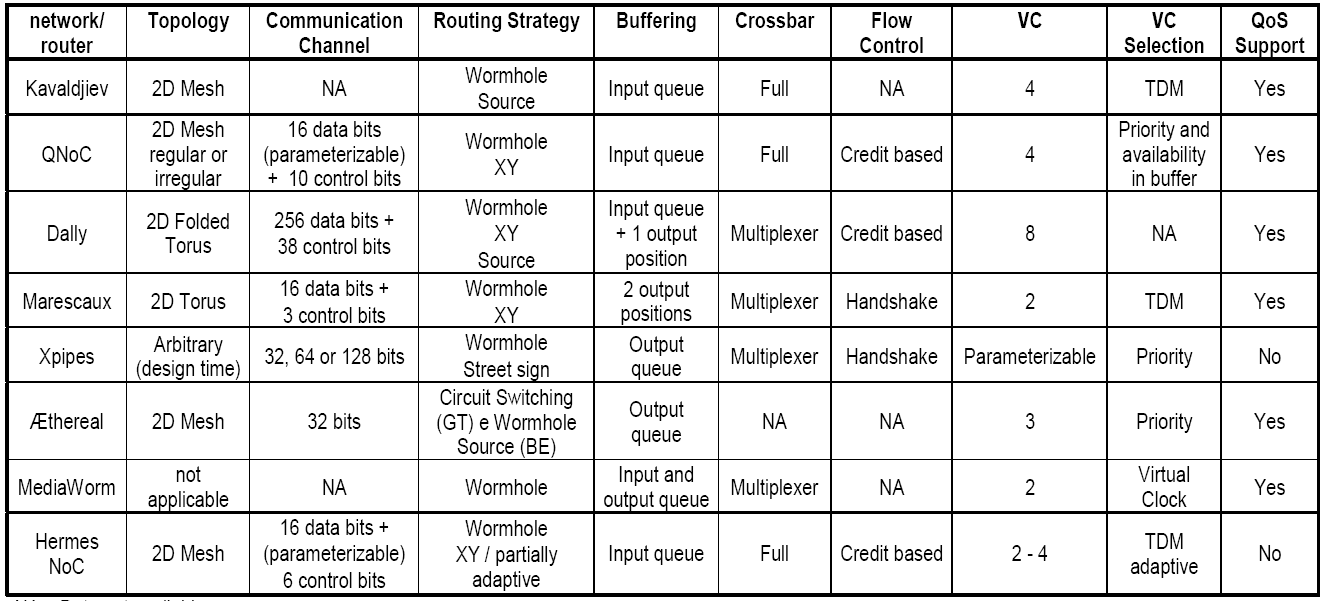
\includegraphics[width=12cm]{OtherArcs.png}
From this we can consider the format of a data packet since we have the 
tradeoff between the length of a packet and the bounded delay of the packet. 
If the packet is long, then our network is more efficient, however, the bounded 
delay will probably large.
\subsection{Routing}
When a reservation path packet reaches a node and the calculated routing link 
to another router cannot afford the service time and transmission rate or delay 
bound for that reserving flow. What should the router do:

\begin{table}[h]
\begin{center}
  \begin{tabular}{ | p{3cm} | p{4cm} | p{4cm} |}
    \hline
	Options & Advantage & Disadvantage \\ \hline
	Backtrack to the source node (router) & 
	Possible find another better path in another direction &
	Possibly cannot find a path \\ \hline
	Backtrack to current node (router) and try another link (direction) &
	- Possibly to find another path (maybe longer).  

	- Can always find a path if the path exists using exhaust search	&
	- The overhead for finding another path using exhaust search is potentially  big.

	- The algorithm routing can be complicated and expensive if implemented in hardware. \\
    \hline
  \end{tabular}
\end{center}
\caption{Routing Considerations}
\label{table:RoutingConsiderations}
\end{table}

Furthermore, should we employ routing able mechanism, this means that a table 
is used at each node to store the information like left utilization $\frac{S}{T}$ at 
each link and delay bound at each link from source to destination or we can 
use some dynamic routing protocols like dynamic source routing (DSR) as in wireless networks.

\section{Implementation}
The router architecture can be implemented as in \cite{Rexford98arouter, Zhang_1service} 
and extend \cite{PehDelayModel, PehSpecPipeR} to have better performance.

We use Noxim \cite{Noxim} as the implementation platform. Currently, we have tried
to set up real-time paths and admission control for real-time paths when sharing 
the same link. The real-time packets currently just contain one flit.

\bibliography{RTNoC}
\bibliographystyle{plain}

\end{document}
